\section{Requisiti funzionali}

%\subsection{Use Case Stories}

I requisiti funzionali sono stati esplicitati mediante le \textit{use case stories}, considerando come attori coinvolti nel sistema: 
\begin{itemize}
	\item Amministratore;
	\item Cliente;
	\item Cuoco;
	\item Cassiere.
\end{itemize}


\subsection{Use case stories: Amministratore}
L’amministratore è un responsabile di sala, col compito di configurare il software nelle fasi di setup dell’attività.
\subsubsection{CONFIGURAZIONE DISPOSITIVI SALA} 
\begin{itemize}
	\item Come amministratore, voglio poter registrare i dispositivi destinati ai tavoli dei clienti per consentire ai commensali di accedere al sistema;
	\item Come amministratore, voglio poter registrare i dispositivi destinati alla cucina per permettere alla cucina di gestire gli ordini;
	\item Come amministratore, voglio poter registrare un dispositivo destinato al cassiere affinché sia possibile elencare al cliente la comanda che ha ordinato.
\end{itemize}

\subsubsection{LOGIN/LOGOUT} 
\begin{itemize}
	\item Come amministratore, voglio poter effettuare il log-in/log-out dal sistema.
\end{itemize}

\subsubsection{CONFIGURAZIONE MENÙ} 
\begin{itemize}
	\item Come amministratore, voglio poter effettuare una gestione del menù per visualizzare/modificare/aggiungere/eliminare portate;  
	\item Come amministratore, voglio poter aggiungere/rimuovere/modificare gli ingredienti assegnati ad una portata per dettagliare la composizione.
\end{itemize}


\subsection{Use case stories: Cliente}
Il cliente può essere di due tipi: il cliente al tavolo, che usufruisce del dispositivo posto a disposizione dal ristorante, e il cliente da asporto, che comunica la sua ordinazione al ristorante tramite un portale sulla rete.

\subsubsection{AUTENTICAZIONE} 
\begin{itemize}
	\item Come cliente, voglio che il sistema riconosca i miei ordini così che possa elaborare le informazioni relative alla mia comanda;
\end{itemize}

\subsubsection{VISUALIZZARE MENÙ} 
\begin{itemize}
	\item Come cliente, voglio poter visualizzare il menù per decidere quale pietanza ordinare.
\end{itemize}

\subsubsection{EFFETTUARE UN'ORDINAZIONE} 
\begin{itemize}
	\item Come cliente, voglio effettuare un’ordinazione per ottenere una o più pietanze; 
	\item Come cliente, voglio effettuare un’ordinazione personalizzando la pietanza desiderata per, ad esempio, togliere ingredienti non desiderati.
\end{itemize}

\subsubsection{VISUALIZZARE STATO ORDINI} 
\begin{itemize}
	\item Come cliente, voglio poter visualizzare lo stato di preparazione dei miei ordini per poter avere un feedback dalla cucina.
\end{itemize}

\subsubsection{ANNULLARE UN ORDINE} 
\begin{itemize}
	\item Come cliente, voglio annullare l’ordinazione di un piatto.
\end{itemize}

\subsubsection{MODIFICARE UN ORDINE} 
\begin{itemize}
	\item Come cliente al tavolo, voglio poter modificare un ordine già mandato verso la cucina per, ad esempio, precisare ingredienti da togliere, qualora l’ordine non fosse già in preparazione;
	\item Come cliente al tavolo, voglio poter modificare un ordine già mandato verso al cucina per, ad esempio, esigere il piatto prima (ad es., se il cliente ritiene di star aspettando troppo) o posticipare la sua preparazione.
\end{itemize}

\subsection{Use case stories: Cuoco}
Il terzo attore coinvolto è il cuoco che prepara le ordinazioni col supporto del sistema.
\subsubsection{GESTIONE PREPARAZIONE ORDINI} 
\begin{itemize}
	\item come cuoco, voglio poter gestire gli ordini effettuati dai clienti per poter eventualmente gestire la priorità di essi;
	\item come cuoco, voglio poter modificare lo stato di un piatto per avvertire il sistema di un’avvenuta preparazione.
\end{itemize}

\subsubsection{VISUALIZZAZIONE LISTA ORDINI} 
\begin{itemize}
	\item Come cuoco, voglio poter verificare lo stato degli ordini richiesti.
\end{itemize}

\subsection{Use case stories: Cassiere}
Il cassiere legge la comanda del cliente al fine di elencare le pietanze da lui ordinate, dettagliare informazioni annesse e calcolarne il conto.
\subsubsection{VISUALIZZARE COMANDA} 
\begin{itemize}
	\item Come cassiere, voglio visualizzare la comanda delle ordinazioni relativa a un determinato cliente per generare il conto.
\end{itemize}

\subsubsection{GENERAZIONE CONTO} 
\begin{itemize}
	\item Come cassiere, voglio poter generare il conto per un determinato cliente, per concludere la sua sessione nel sistema.
	
\end{itemize}


\subsection{Priorità dei casi d’uso}

Per ottimizzare il processo di sviluppo, si è deciso di categorizzare le specifiche funzionali in tabelle con tre livelli di priorità: elevata, media e bassa. Nello specifico il primo livello è assegnato alla Tabella~\ref{tab:use_cases_high_priority} a cui sono attribuiti i casi d'uso essenziali per il funzionamento dell'applicazione, i casi d'uso relativi alle funzionalità aggiuntive non critiche sono stati attribuiti alla Tabella~\ref{tab:use_cases_medium_priority} a priorità media, mentre il livello a bassa priorità che accoglie requisiti funzionali opzionali previsti per versioni successive alla Tabella~\ref{tab:use_cases_low_priority} .

\clearpage
\subsubsection{PRIORITÀ ELEVATA}

\begin{table}[htbp]
	\centering
	 \begin{tabularx}{\textwidth}{|>{\centering\arraybackslash} m{4em}| >{\raggedright\arraybackslash}X |}
		\hline
		\textbf{Codice} & \textbf{Titolo} \\ [0.5ex]
		\hline\hline
		UC1 & Gestione comanda  \\
		\hline
		UC2 & Effettuare un'ordinazione \\
		\hline
		UC3 & Visualizzare menù \\
		\hline
		UC4 & Autenticazione \\
		\hline
		UC5 & Visualizzare lista ordini \\
		\hline
		UC6 & Gestione preparazione ordini \\
		\hline
	\end{tabularx}
	\caption{Casi d'uso ad elevata priorità}
	\label{tab:use_cases_high_priority}
\end{table}

\subsubsection{PRIORITÀ MEDIA}
\begin{table}[htbp]
	\centering
	\begin{tabularx}{\textwidth}{|>{\centering\arraybackslash} m{4em}| >{\raggedright\arraybackslash}X |}
		\hline
		\textbf{Codice} & \textbf{Titolo} \\ [0.5ex]
		\hline\hline
		UC7 & Configurazione dispositivi sala \\
		\hline
		UC8 & Gestione dispositivi \\
		\hline
		UC9 & Login amministratore \\
		\hline
		UC10 & Logout amministratore \\
		\hline
		UC11 & Configurazione menù \\
		\hline
		UC12 & Gestione dati menù \\
		\hline
	\end{tabularx}
	\caption{Casi d'uso a media priorità}
	\label{tab:use_cases_medium_priority}
\end{table}

\subsubsection{PRIORITÀ BASSA}
\begin{table}[htbp]
	\centering
	\begin{tabularx}{\textwidth}{|>{\centering\arraybackslash} m{4em}| >{\raggedright\arraybackslash}X |}
		\hline
		\textbf{Codice} & \textbf{Titolo} \\ [0.5ex]
		\hline\hline
		UC13 & Modifica un ordine  \\
		\hline
		UC14 & Annullare un ordine  \\
		\hline
		UC15 & Visualizza stato delle ordinazioni \\
		\hline
		UC16 & Generazione conto   \\
		\hline
		UC17 & Visualizzare comanda   \\
		\hline
	\end{tabularx}
	\caption{Casi d'uso a bassa priorità}
	\label{tab:use_cases_low_priority}
\end{table}


\subsection{Use case diagram}

Dalla descrizione delle \textit{use case stories}, è stato creato il diagramma UML dei casi d'uso in \figurename~\ref{fig:use_cases_diagram}, il quale è composto da 4 attori (Amministratore, Cuoco, Cassiere e Cliente che tramite ereditarietà viene ridefinito in Cliente al tavolo oppure Cliente che effettua ordinazioni d’asporto) e 6 viste (vista amministratore, vista cucina, vista cassiere, vista cliente, vista cliente al tavolo e sistema).

\begin{figure}[htbp]
	\begin{comment}
		The [htbp] option in LaTeX is used to fine-tune the placement of tables and figures.
		Each letter in [htbp] stands for a particular placement option:
		h (here): Place the table or figure in the text where the environment (like figure or table) is written, if there is enough room left on the page.
		t (top): Place it at the top of a page.
		b (bottom): Place it at the bottom of a page.
		p (page): Place it on a page containing only floats, such as figures and tables	
		LaTeX will try to place the float at the location that comes first in the option list.
		If it can’t place it there due to constraints like page size, it will move on to the next option. If none of the specified options work, LaTeX will hold the float until it finds a place where it fits, or until a \clearpage command is encountered
	\end{comment}
	\centering
	
	% verticale
	%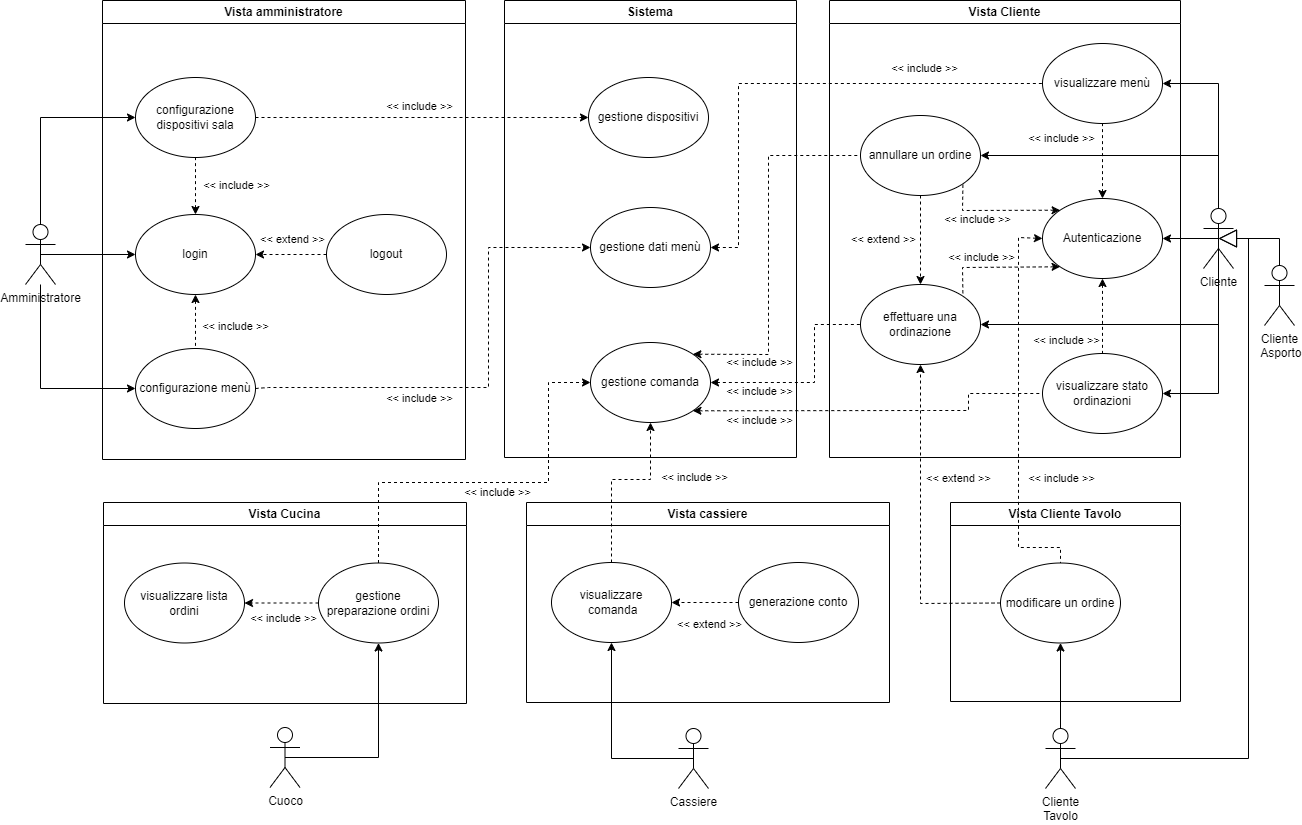
\includegraphics[scale=0.4, angle=90]{iterazione0/images/use_cases_diagram}
	
	% orizzontale
	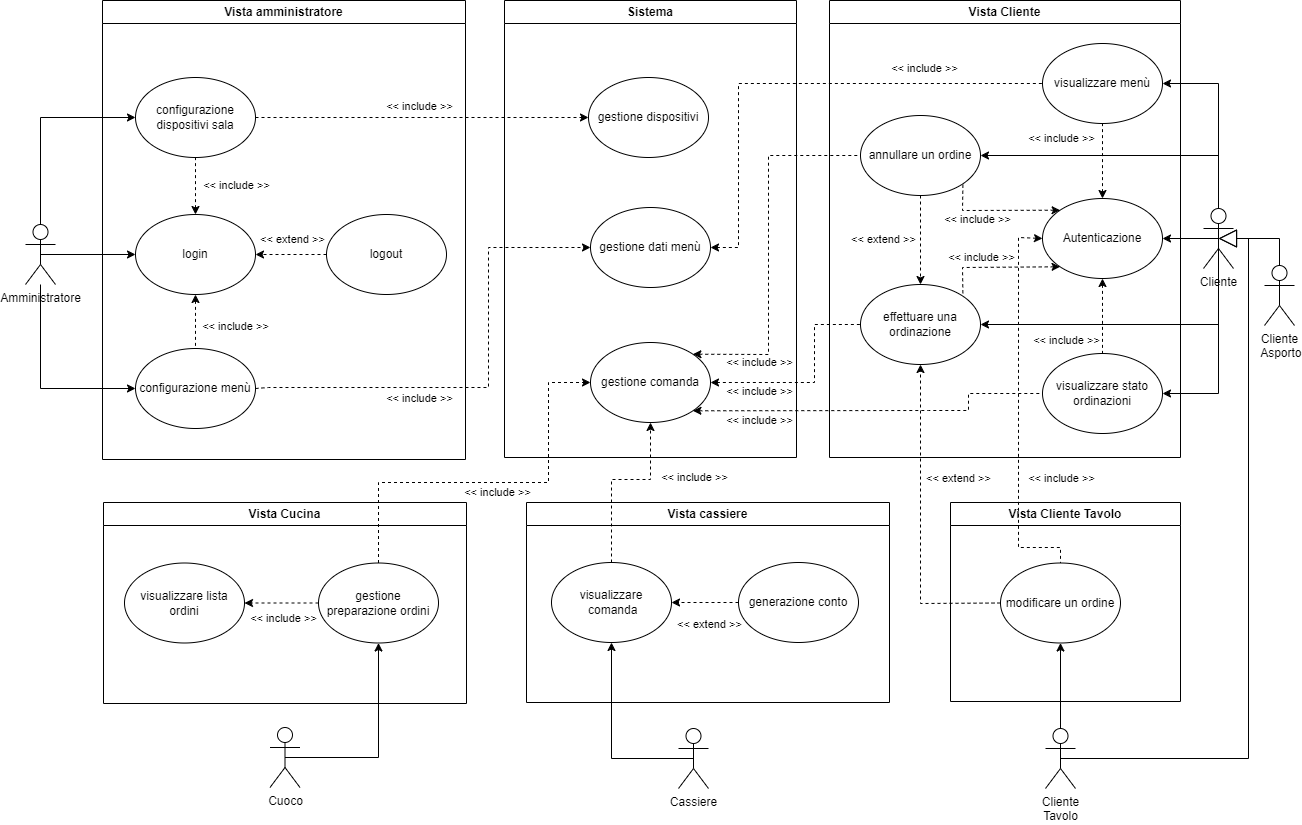
\includegraphics[scale=0.32]{iterazione0/images/use_cases_diagram}
	\caption{Diagramma dei casi d'uso\label{fig:use_cases_diagram}}
\end{figure}

\clearpage